%!TEX root = ../thesis.tex

\subsection{RRM(Random Road Map)}

\begin{figure}[hbtp]
  \centering
 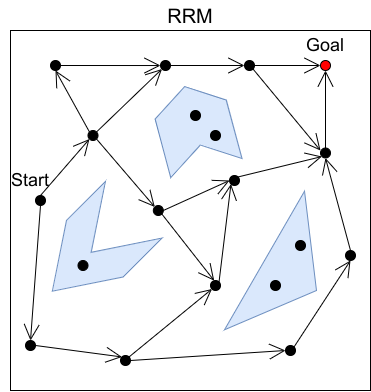
\includegraphics[keepaspectratio, scale=0.8]
      {images/png/RRT.drawio.png}
 \caption{RRM}
 \label{Fig:RRM}
\end{figure}

RRMはランダムにSeedsと呼ばれる点をばらまき,
障害物の内部のSeedsは考えずにその他の点を結んでグラフを作り経路を計画する手法である.
Fig.\ref{Fig:RRM}はRRMのイメージ図である.黒い点がSeeds,水色の図形が障害物,矢印が経路である.
このようにランダムに配置されたSeedsの内,障害物内のものを除いて接続していき経路を生成する.

問題点としては,計算量が多いことと,通る場所が狭いときに更に計算時間がかかることである.
この問題点を解決するためにRRTなどの改良版のアルゴリズムが存在する.

\newpage
